\subsubsection{\texttt{RF-11}: iconos de color para ejercicios}
\label{subsec:rf11}

Las aplicaciones que cuentan con GUI, como es el caso de \textit{VSCode4Teaching}, requieren que la interacción entre el usuario y los componentes que emplean sea lo más intuitiva y sencilla posible, buscando mostrar la información solicitada de forma clara y ágilmente interpretable, disponiendo los elementos necesarios para que el usuario actúe en consecuencia intercambiando nueva información con la aplicación, conduciendo a un uso fluido que satisfaga sus necesidades. Este hecho viene apoyado por el objetivo cuarto del Trabajo Fin de Grado ---véase el \referenciaCapitulo{cap:objetivos}---, que especifica que se deben incorporar mejoras visuales en la interfaz de usuario para facilitar el uso de la aplicación.

Gracias a la implementación del presente requisito, todos los usuarios de la aplicación ---con independencia de su rol--- visualizrán un nuevo icono junto a cada uno de los ejercicios disponibles.

Como la información que busca reflejar el icono es distinta para cada uno de los roles ---y, en consonancia, el propio icono---, se establecen dos requisitos derivados:
\begin{itemize}
    \item El requisito \texttt{RF-11.1} es el destinado a los estudiantes, estableciendo que el icono debe mostrar el estado en que se encuentra el ejercicio (pudiendo ser ``no comenzado'', ``en progreso'' o ``finalizado''). En la \referenciaFigura{fig:reqf11-1} se pueden apreciar los iconos mostrados a los estudiantes (en la parte izquierda): el ejercicio ``ej8'' tiene asociado el icono verde, asociado al último estado; ``ej9'', el icono amarillo ---reflejando estado ``en progreso''---; y ``ej7'', el icono rojo, que indica que el estudiante no ha comenzado el ejercicio.
    \item Análogamente, el requisito \texttt{RF-11.2} fija que los profesores visualicen un icono que aluda a la existencia de una solución adjunta al ejercicio y, en caso de haberla, que indique su disponibilidad. La \referenciaFigura{fig:reqf11-1} (en la parte derecha) ilustra los tres iconos disponibles para mostrar junto a cada ejercicio: el icono amarillo del ejercicio ``ej9'' indica que no tiene solución asociada; el rojo del ejercicio ``ej7'', que la solución adjunta no es pública; y el verde del ejercicio ``ej8'', que la solución ha sido publicada a los estudiantes.
\end{itemize}

Asimismo, la semántica de estos iconos también se refleja en el \textit{tooltip}\footnote{\textit{Tooltip}. Es un elemento textual que aparece en la interfaz de usuario cuando este mantiene el cursor encima de un ejercicio sin presionarlo durante varios segundos.}, en el que los estudiantes pueden visualizar entre paréntesis el estado del ejercicio en formato textual; y los docentes, una descripción sobre el estado de existencia y disponibilidad de la solución.

\begin{figure}[!ht]
    \centering
    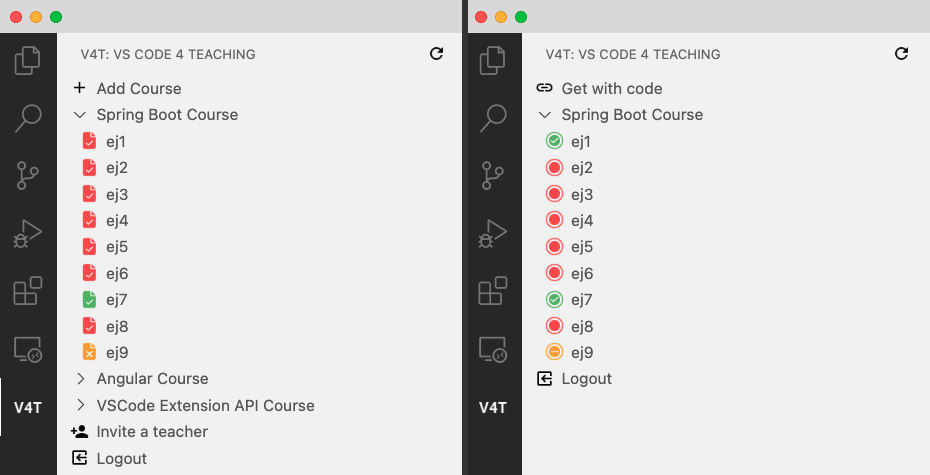
\includegraphics[width=\textwidth]{imagenes/utilizadas/4-3-implementacion/rf11-1.png}
    \caption{Iconos mostrados junto a cada ejercicio para los estudiantes (izquierda) y profesores (derecha).}
    \label{fig:reqf11-1}
\end{figure}
